%%%%%%%%%%%%%%%%%%%%%%%%%%%%%%%%%%%%%%%%%
% Beamer Presentation
% LaTeX Template
% Version 1.0 (10/11/12)
%
% This template has been downloaded from:
% http://www.LaTeXTemplates.com
%
% License:
% CC BY-NC-SA 3.0 (http://creativecommons.org/licenses/by-nc-sa/3.0/)
%
%%%%%%%%%%%%%%%%%%%%%%%%%%%%%%%%%%%%%%%%%

%----------------------------------------------------------------------------------------
%	PACKAGES AND THEMES
%----------------------------------------------------------------------------------------

\documentclass{beamer}

\mode<presentation> {

% The Beamer class comes with a number of default slide themes
% which change the colors and layouts of slides. Below this is a list
% of all the themes, uncomment each in turn to see what they look like.

%\usetheme{default}
%\usetheme{AnnArbor}
%\usetheme{Antibes}
%\usetheme{Bergen}
%\usetheme{Berkeley}
%\usetheme{Berlin}
%\usetheme{Boadilla} %maybe
%\usetheme{CambridgeUS}
%\usetheme{Copenhagen}
%\usetheme{Darmstadt} %maybe
%\usetheme{Dresden}
%\usetheme{Frankfurt}
%\usetheme{Goettingen} %mit anderem Farbschema maybe
%\usetheme{Hannover} %wie Goettingen nur links maybe
%\usetheme{Ilmenau}
%\usetheme{JuanLesPins}
%\usetheme{Luebeck}
%\usetheme{Madrid}
%\usetheme{Malmoe}
\usetheme{Marburg} %wie Goettingen nur geiler maybe
%\usetheme{Montpellier}
%\usetheme{PaloAlto}
%\usetheme{Pittsburgh}
%\usetheme{Rochester}
%\usetheme{Singapore}
%\usetheme{Szeged}
%\usetheme{Warsaw}

% As well as themes, the Beamer class has a number of color themes
% for any slide theme. Uncomment each of these in turn to see how it
% changes the colors of your current slide theme.

%\usecolortheme{albatross}
%\usecolortheme{beaver}
%\usecolortheme{beetle}
%\usecolortheme{crane}
%\usecolortheme{dolphin}
%\usecolortheme{dove}
%\usecolortheme{fly}
\usecolortheme{lily} %maybe
%\usecolortheme{orchid}
%\usecolortheme{rose}
%\usecolortheme{seagull}
%\usecolortheme{seahorse}
%\usecolortheme{whale}
%\usecolortheme{wolverine}

%\setbeamertemplate{footline} % To remove the footer line in all slides uncomment this line
%\setbeamertemplate{footline}[page number] % To replace the footer line in all slides with a simple slide count uncomment this line

%\setbeamertemplate{navigation symbols}{} % To remove the navigation symbols from the bottom of all slides uncomment this line
}

\usepackage{graphicx} % Allows including images
\usepackage{booktabs} % Allows the use of \toprule, \midrule and \bottomrule in tables
\usepackage[utf8]{inputenc}
\usepackage{dsfont}
\usepackage{cellspace}
\usepackage{todonotes}
%----------------------------------------------------------------------------------------
%	TITLE PAGE
%----------------------------------------------------------------------------------------

\title[Ägyptische Brüche]{Darstellung rationaler Zahlen durch Ägyptische Brüche} % The short title appears at the bottom of every slide, the full title is only on the title page

\author{Lars Berger} % Your name
\institute[UniBwM]{Universität der Bundeswehr München}
\date{18. Dezember 2019} % Date, can be changed to a custom date



\begin{document}
\newcommand{\R}{\mathds{R}}
\newcommand{\Z}{\mathds{Z}}
\newcommand{\N}{\mathds{N}}
\newcommand{\Q}{\mathds{Q}}
\newcommand{\K}{\mathds{K}}
\newcommand{\C}{\mathds{C}}
\newcommand{\B}{\mathds{B}}
\newcommand{\F}{\mathds{F}}
\newcommand{\p}{\mathfrak{p}}
\newcommand{\Pot}{\mathcal{P}}
\newcommand{\id}{\textup{id}}
\newcommand{\Ker}{\textup{Ker}}
\newcommand{\Image}{\textup{Im}}
\newcommand{\la}{\langle}
\newcommand{\ra}{\rangle}
\newcommand{\gdw}{\Leftrightarrow}
\newcommand{\uf}[1]{\frac{1}{#1}}

\begin{frame}
\titlepage % Print the title page as the first slide
\end{frame}

\begin{frame}
\frametitle{Inhalt}
\tableofcontents
\end{frame}

\section{Einführung}
\begin{frame}
	\begin{block}{Definition}
	Ein Bruch soll fortan ,,in ägyptischer Form'' bzw. ,,Ägyptischer Bruch'' heißen genau dann, wenn er in der Form
	$$\uf{x_1} + \uf{x_2} + \cdots + \uf{x_n}, \quad n \in \N, n \ge 1$$
	mit paarweise verschiedenen $x_i, \, i \in \left\{1,...,n\right\}$, vorliegt.
	\end{block}
\end{frame}

\subsection{Geschichte}

\subsection{Ägyptische Multiplikation}
%\setbeamercovered{invisible}
\begin{frame}
	\frametitle{Ägyptische Multiplikation}
	\begin{block}{Beispiel: $23\cdot69$}
		\centering
		\begin{tabular}{c r r}
			\only<5->{$\checkmark$}&1&69\\
			\only<4->{$\checkmark$}&2&138\\
			\only<3->{$\checkmark$}&4&276\\
			&8&552\\
			\only<2->{$\checkmark$}&16&1104\\ \hline
			Summe:&\only<1>{0&0}\only<2>{16&1104}\only<3>{20&1380}\only<4>{22&1518}\only<5->{23&1587}\\
		\end{tabular}
	\end{block}
\end{frame}

\subsection{Ägyptische Division}
\begin{frame}
\frametitle{Ägyptische Division}
	\begin{block}{Beispiel: $117 \div 7$}
		\centering
		\begin{tabular}{Sc Sr Sr}
			&1&7\\
			&2&14\\
			&4&28\\
			&8&56\\
			\only<2->{$\checkmark$}&16&112\\ \hline
			Summe:&\only<1>{0&0}\only<2->{16&112}\\
		\end{tabular}
	\end{block}
\end{frame}

\begin{frame}
\frametitle{Ägyptische Division}
		\centering
		\begin{tabular}{Sr Sr}
			1 & 7\\
			$\uf{7}$ & $1$\\
			$\uf{14}$ & $\uf{2}$\\
			$\uf{28}$ & $\uf{4}$\\
			$\vdots$ & $\vdots$ \\
		\end{tabular}
		\qquad \quad
		\begin{tabular}{c | c}
			&\\&\\&\\&\\&\\&\\
		\end{tabular}
		\qquad
		\begin{tabular}[h]{Sr Sr}
			$1$ & $7$\\
			$\uf{2}$ & $3+\uf{2}$\\
			$\uf{4}$ & $1+\uf{2}+\uf{4}$\\
			$\uf{8}$ & $\uf{2}+\uf{4}+\uf{8}$\\
			$\vdots$&$\vdots$\\
		\end{tabular}
\end{frame}

\begin{frame}
\frametitle{Ägyptische Division}
	\begin{block}{Beispiel: $117 \div 7$}
		\centering
		\begin{tabular}{Sc Sr Sr}
			&1&7\\
			&2&14\\
			&4&28\\
			&8&56\\
			$\checkmark$&16&112\\
			\only<2->{$\checkmark$}&$\uf{2}$&$3+\uf{2}$\\
			\only<3->{$\checkmark$}&$\uf{7}$&$1$\\
			\only<4->{$\checkmark$}&$\uf{14}$&$\uf{2}$\\ \hline
			Summe:&\only<1>{16&112}\only<2>{$16+\uf{2}$&$115+\uf{2}$}\only<3>{$16+\uf{2}+\uf{7}$&$116+\uf{2}$}\only<4->{$16+\uf{2}+\uf{7}+\uf{14}$&$117$}\\
		\end{tabular}
	\end{block}
\end{frame}

\section{Zerlegungsalgorithmen}

\begin{frame}
\frametitle{Zerlegungsalgorithmen}
Betrachtung einer Auswahl:
	\begin{itemize}
		\item Greedy-Algortihmus
		\item Farey-Folgen-Algorithmus
		\item Binäralgorithmus
	\end{itemize}
\end{frame}

\subsection{Greedy-Algorithmus}

\begin{frame}
	\frametitle{Der Greedy-Algorithmus}
	\begin{block}{Ziel}
		$$\frac{a}{b} = \frac{1}{x_1} + \frac{1}{x_2} + ... + \frac{1}{x_i} = \sum_{j=1}^{i} \frac{1}{x_j}.$$
	\end{block}
	\begin{block}{Algorithmus}<2->
		\begin{enumerate}
			\item finde den größten, noch nicht verwendeten Stammbruch $\uf{x}$, sodass $\uf{x} \leq \frac{p}{q}$.
			\item setze $\uf{x}$ als weiteren Summanden des Ergebnisses
			\item falls $\frac{p}{q} - \uf{x} > 0$, gehe zu Schritt 1 mit $\left(\frac{p}{q}\right) \leftarrow \left(\frac{p}{q}-\uf{x}\right)$.
		\end{enumerate}
	\end{block}
\end{frame}

\begin{frame}
	\frametitle{Der Greedy-Algorithmus: Rechenbeispiel}
	Gesucht: Zerlegung für $\frac{5}{9}$.
	$$\frac{5}{9}\only<3-4>{>}\only<5->{=}\only<3->{\uf{2}}\only<5->{+\uf{18}}$$
	\only<-4>{Nebenrechnungen:}
	\only<2-3>{$$\uf{2} \leq \frac{5}{9} < \uf{1}$$}
	\only<4>{$$\frac{5}{9} - \uf{2} = \uf{18}$$}
\end{frame}

%\begin{frame}
%	\frametitle{Der Greedy-Algorithmus: Rechenbeispiel}
%	Gesucht: Zerlegung für $\frac{24}{31}$.\\
%	\begin{center}
%		$\frac{24}{31}$ \only<-10>{$>$}\only<11->{$=$} $\only<1-2>{0}\only<3->{\uf{2}}\only<6->{+\uf{4}}\only<9->{+\uf{42}}\only<11->{+\uf{2604}}$
%	\end{center}
%	\only<-10>{Nebenrechnungen:\\}
%	\begin{center}
%		\only<2-3>{$\uf{2}\leq \frac{24}{31} < \uf{1}$}
%		\only<4>{$\frac{24}{31} - \uf{2} = \frac{17}{62}$}
%		\only<5-6>{$\uf{4}\leq \frac{17}{62} < \uf{3}$}
%		\only<7>{$\frac{17}{62} - \uf{4} = \frac{3}{124}$}
%		\only<8-9>{$\uf{42}\leq \frac{3}{124} < \uf{41}$}
%		\only<10>{$\frac{3}{124} - \uf{42} = \uf{2604}$}
%	\end{center}
%\end{frame}

\subsection{Farey-Folgen-Algorithmus}

\begin{frame}
\frametitle{Farey-Folgen}
	\begin{block}{Definition}
	Sei $q \in \N$. Die Farey-Folge der Ordnung $q$, $\, F_q$, ist definiert als die aufsteigend sortierte Folge aller einmalig darin vorkommenden gekürzten Brüche $\frac{a}{b} \in \Q$, für die gilt:
	$0\leq a \leq b \leq q,\, b\neq 0$.
	\end{block}
	\hspace{5cm}
	\begin{block}{Beispiel: $F_5$}<2->
		$$F_5 = \left(\frac{0}{1}, \uf{5}, \uf{4}, \uf{3}, \frac{2}{5}, \uf{2}, \frac{3}{5}, \frac{2}{3}, \frac{3}{4}, \frac{4}{5}, \uf{1} \right).$$
	\end{block}
\end{frame}

\begin{frame}
	\frametitle{Der Farey-Folgen-Algorithmus}
	\begin{block}{Algorithmus}
		Sei $\frac{p}{q} \in \Q_+$ in gekürzter Form der zu zerlegende Bruch.\\
		\begin{enumerate}
			\item Konstruiere $F_q$.
			\item Sei $\frac{r}{s}$ der zu $\frac{p}{q}$ adjazente Bruch in $F_q$, sodass $\frac{r}{s} < \frac{p}{q}$. Aufgrund der Eigenschaften der Farey-Folge gilt dann
			$$\frac{p}{q} = \uf{qs} + \frac{r}{s},$$ wobei $s<q,\, r<p$.
			\item Wiederhole dieses Vorgehen für $\frac{r}{s}$ solange, bis $s=1 \gdw r=0$.
		\end{enumerate}
	\end{block}
\end{frame}

\begin{frame}
\frametitle{Der Farey-Folgen-Algorithmus: Rechenbeispiel}
	Gesucht: Zerlegung für $\frac{5}{9}$.
	$$\frac{p}{q} = \frac{5}{9} = \uf{qs} + \frac{r}{s}$$\\
	\onslide<2->{$$F_{9rel} = \left( \frac{0}{1}, \uf{2}, \frac{5}{9}, \frac{4}{7}, \frac{3}{5}, \frac{2}{3}, \uf{1}\right)$$} \onslide<3->{$$\Rightarrow\frac{r}{s} = \uf{2}$$}
	\onslide<4->{$$\frac{5}{9} = \uf{9 \cdot 2} + \uf{2} =  \uf{2} + \uf{18}$$}
\end{frame}

\subsection{Binär-Algorithmus}

\begin{frame}
	\frametitle{Der Binäralgorithmus}
	\begin{block}{Algorithmus}
		\only<1>{Sei $\frac{p}{q} \in \Q_+$ in gekürzter Form und $k \in \N$.}
		\begin{enumerate}
			\only<1>{\item Finde $N_{k-1} < q \leq N_k$ wobei $N_k=2^k$ ist.
			\item Falls $q = N_k$, schreibe $p$ als Summe von Teilern von $N_k$, hier $d_i$ genannt:
			$$\frac{p}{q} = \sum_{i=1}^{j} \frac{d_i}{N_k}=  \sum_{i = 1}^{j}\frac{1}{\frac{N_k}{d_i}}$$}
			\only<2>{\setcounter{enumi}{2}\item Sonst seien $s, r \in \N, 0 \leq r < q$ so gewählt, dass:
			$$pN_k = qs+r.$$
			Es folgt:
			$$\frac{p}{q} = \frac{p N_k}{q N_k} = \frac{qs + r}{q N_k} = \frac{s}{N_k} + \frac{r}{q N_k}.$$
			\item Schreibe $s = \sum d_i$ und $r = \sum d_i'$, wobei $d_i, d_i'$ jeweils paarweise verschiedene Teiler von $N_k$ sind.
			\item Erhalte den Ägyptischen Bruch:
			$$\sum \uf{\frac{N_k}{d_i}} + \sum \uf{\frac{q N_k}{d_i'}}.$$}
		\end{enumerate}
	\end{block}

\end{frame}

\begin{frame}
\frametitle{Der Binär-Algorithmus: Rechenbeispiel}
	Gesucht: Zerlegung für $\frac{5}{9}$.
	\onslide<2->{$$8<9<16 \Rightarrow N_k = 16$$\\}
	\begin{center}
		\onslide<3->{$\frac{5}{9}$} \only<4->{$ = \frac{5\cdot16}{9 \cdot 16}$} \only<5->{$ = \frac{9 \cdot 8 + 8}{9 \cdot 16}$} \only<6->{$ = \frac{8}{16} + \frac{8}{144}$} \only<7->{$ = \uf{2} + \uf{18}.$}
	\end{center}
\end{frame}

\section{Auswertung einiger Testreihen}
\subsection{Methodik}
\begin{frame}
	\frametitle{Auswertung von Testreihen: Methodik}
	Datensatzform: $M_q = \left\{ \frac{p}{q} \, | \left(\, 2\leq p < q\right) \wedge \left(\text{ggT}(p,q) = 1\right)\right\}$\\ \vspace{1cm}
	Enthaltene Informationen:
	\begin{itemize}
		\item die durchschnittliche Anzahl der Summanden, \emph{avgTerms(q)}
		\item das Minimum der Anzahl der Summanden, \emph{minTerms(q)}
		\item das Maximum der Anzahl der Summanden, \emph{maxTerms(q)}
		\item das Minimum des jeweils größten Nenners, \emph{minDenom(q)}
		\item das Maximum des jeweils größten Nenners, \emph{maxDenom(q)}.
	\end{itemize}
\end{frame}

\subsection[Ergebnisse]{Nennenswerte Ergebnisse}
\begin{frame}
	\frametitle{Durchschnittliche Anzahl der Terme}
	\begin{figure}[h]
		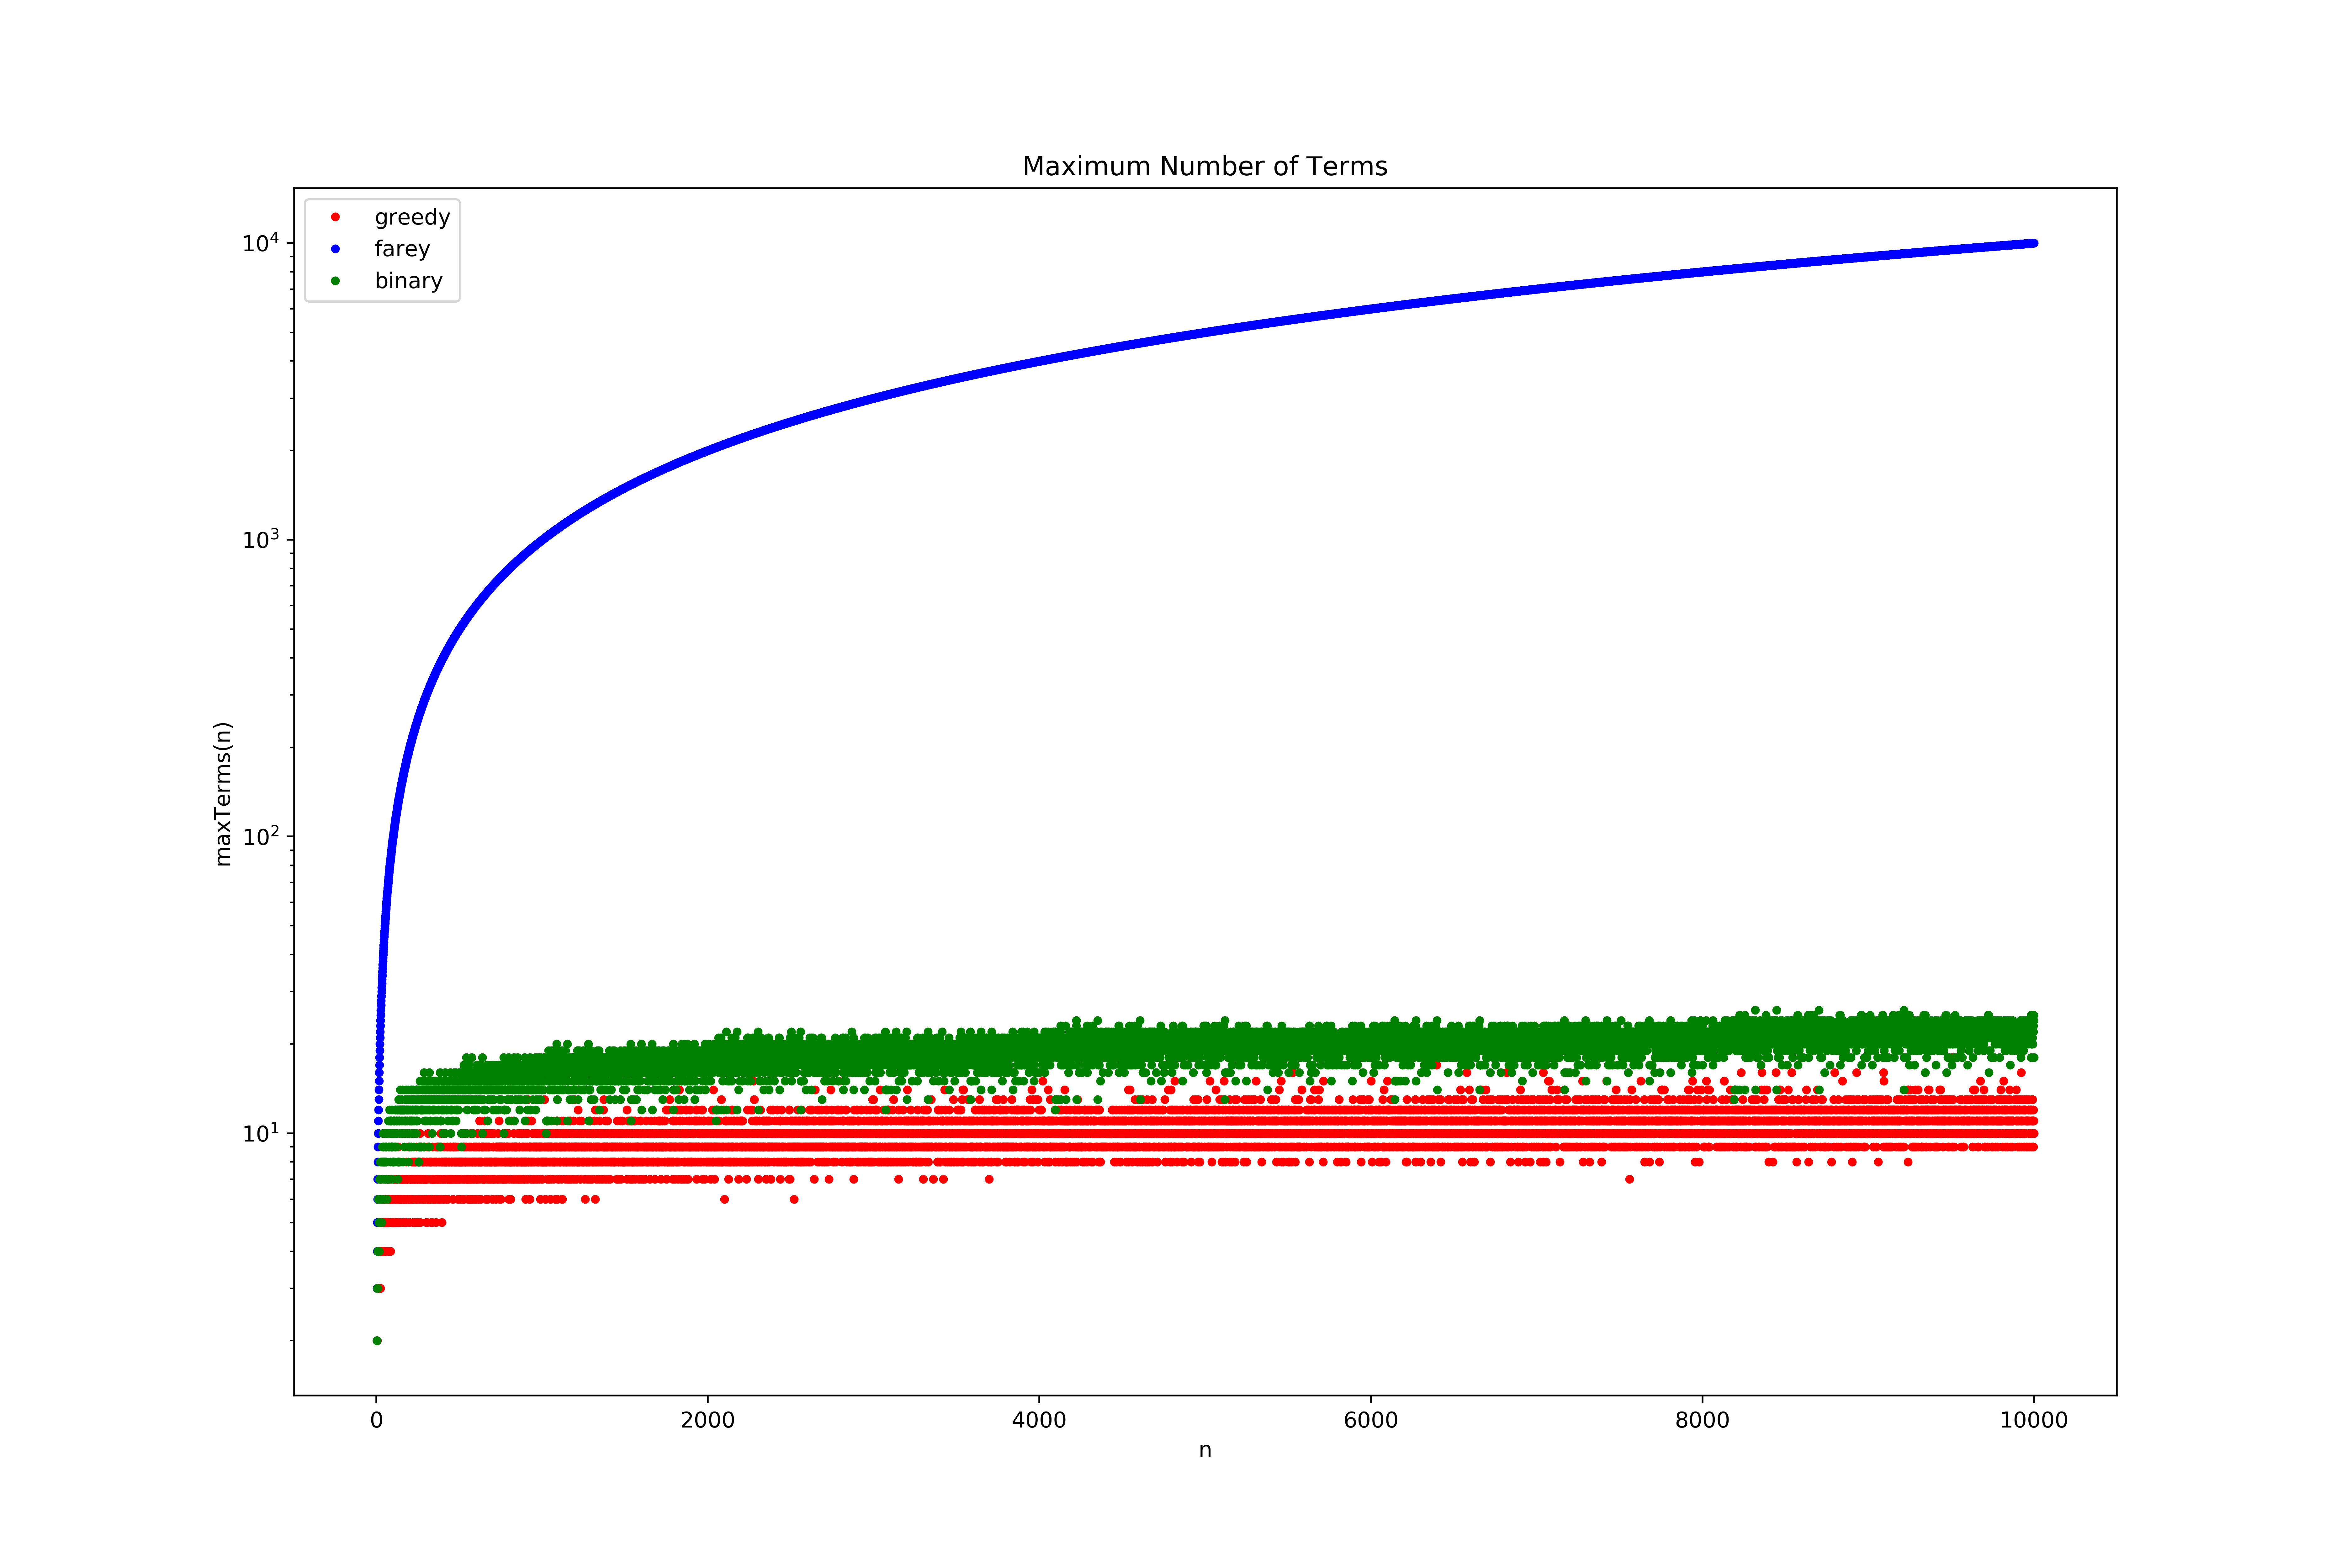
\includegraphics[width=\textwidth]{../LaTeX-Doc/images/maxTerms.png}
	\end{figure}
\end{frame}

\begin{frame}
\frametitle{Minimum der größten Nenner}
\begin{figure}[h]
	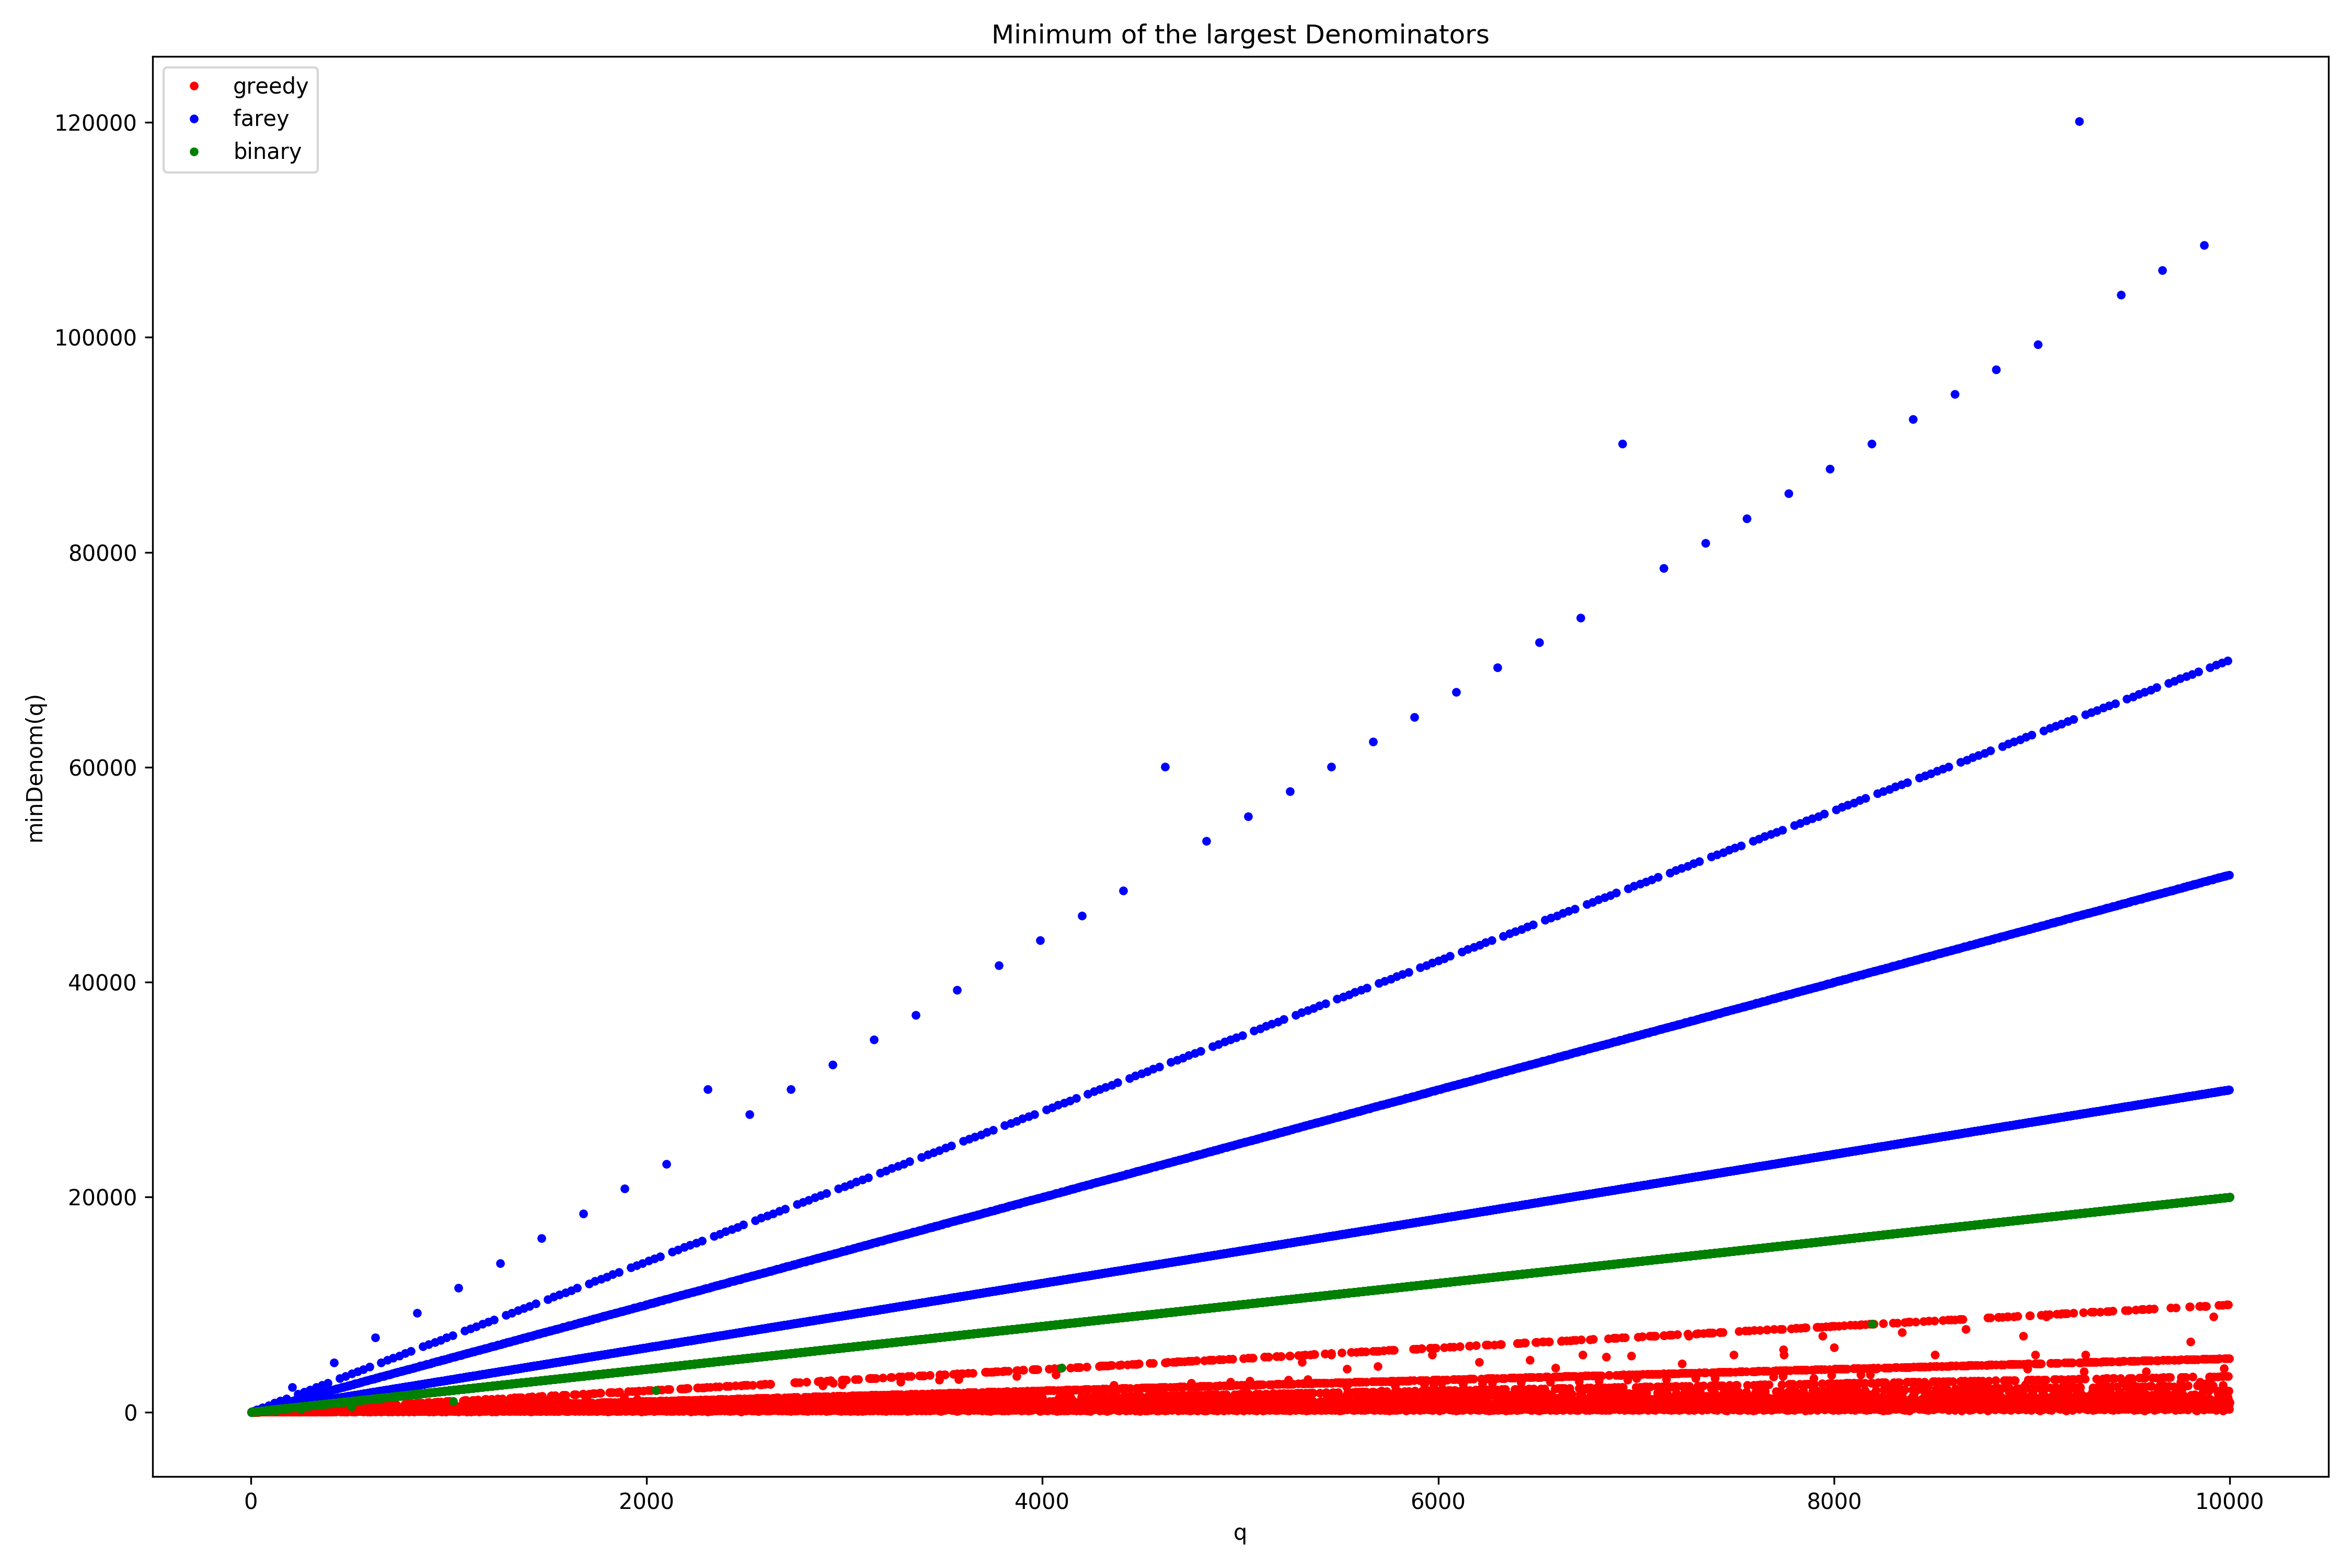
\includegraphics[width=\textwidth]{../LaTeX-Doc/images/minDenom.png}
\end{figure}
\end{frame}

\begin{frame}
\frametitle{Maximum der größten Nenner}
\begin{figure}[h]
	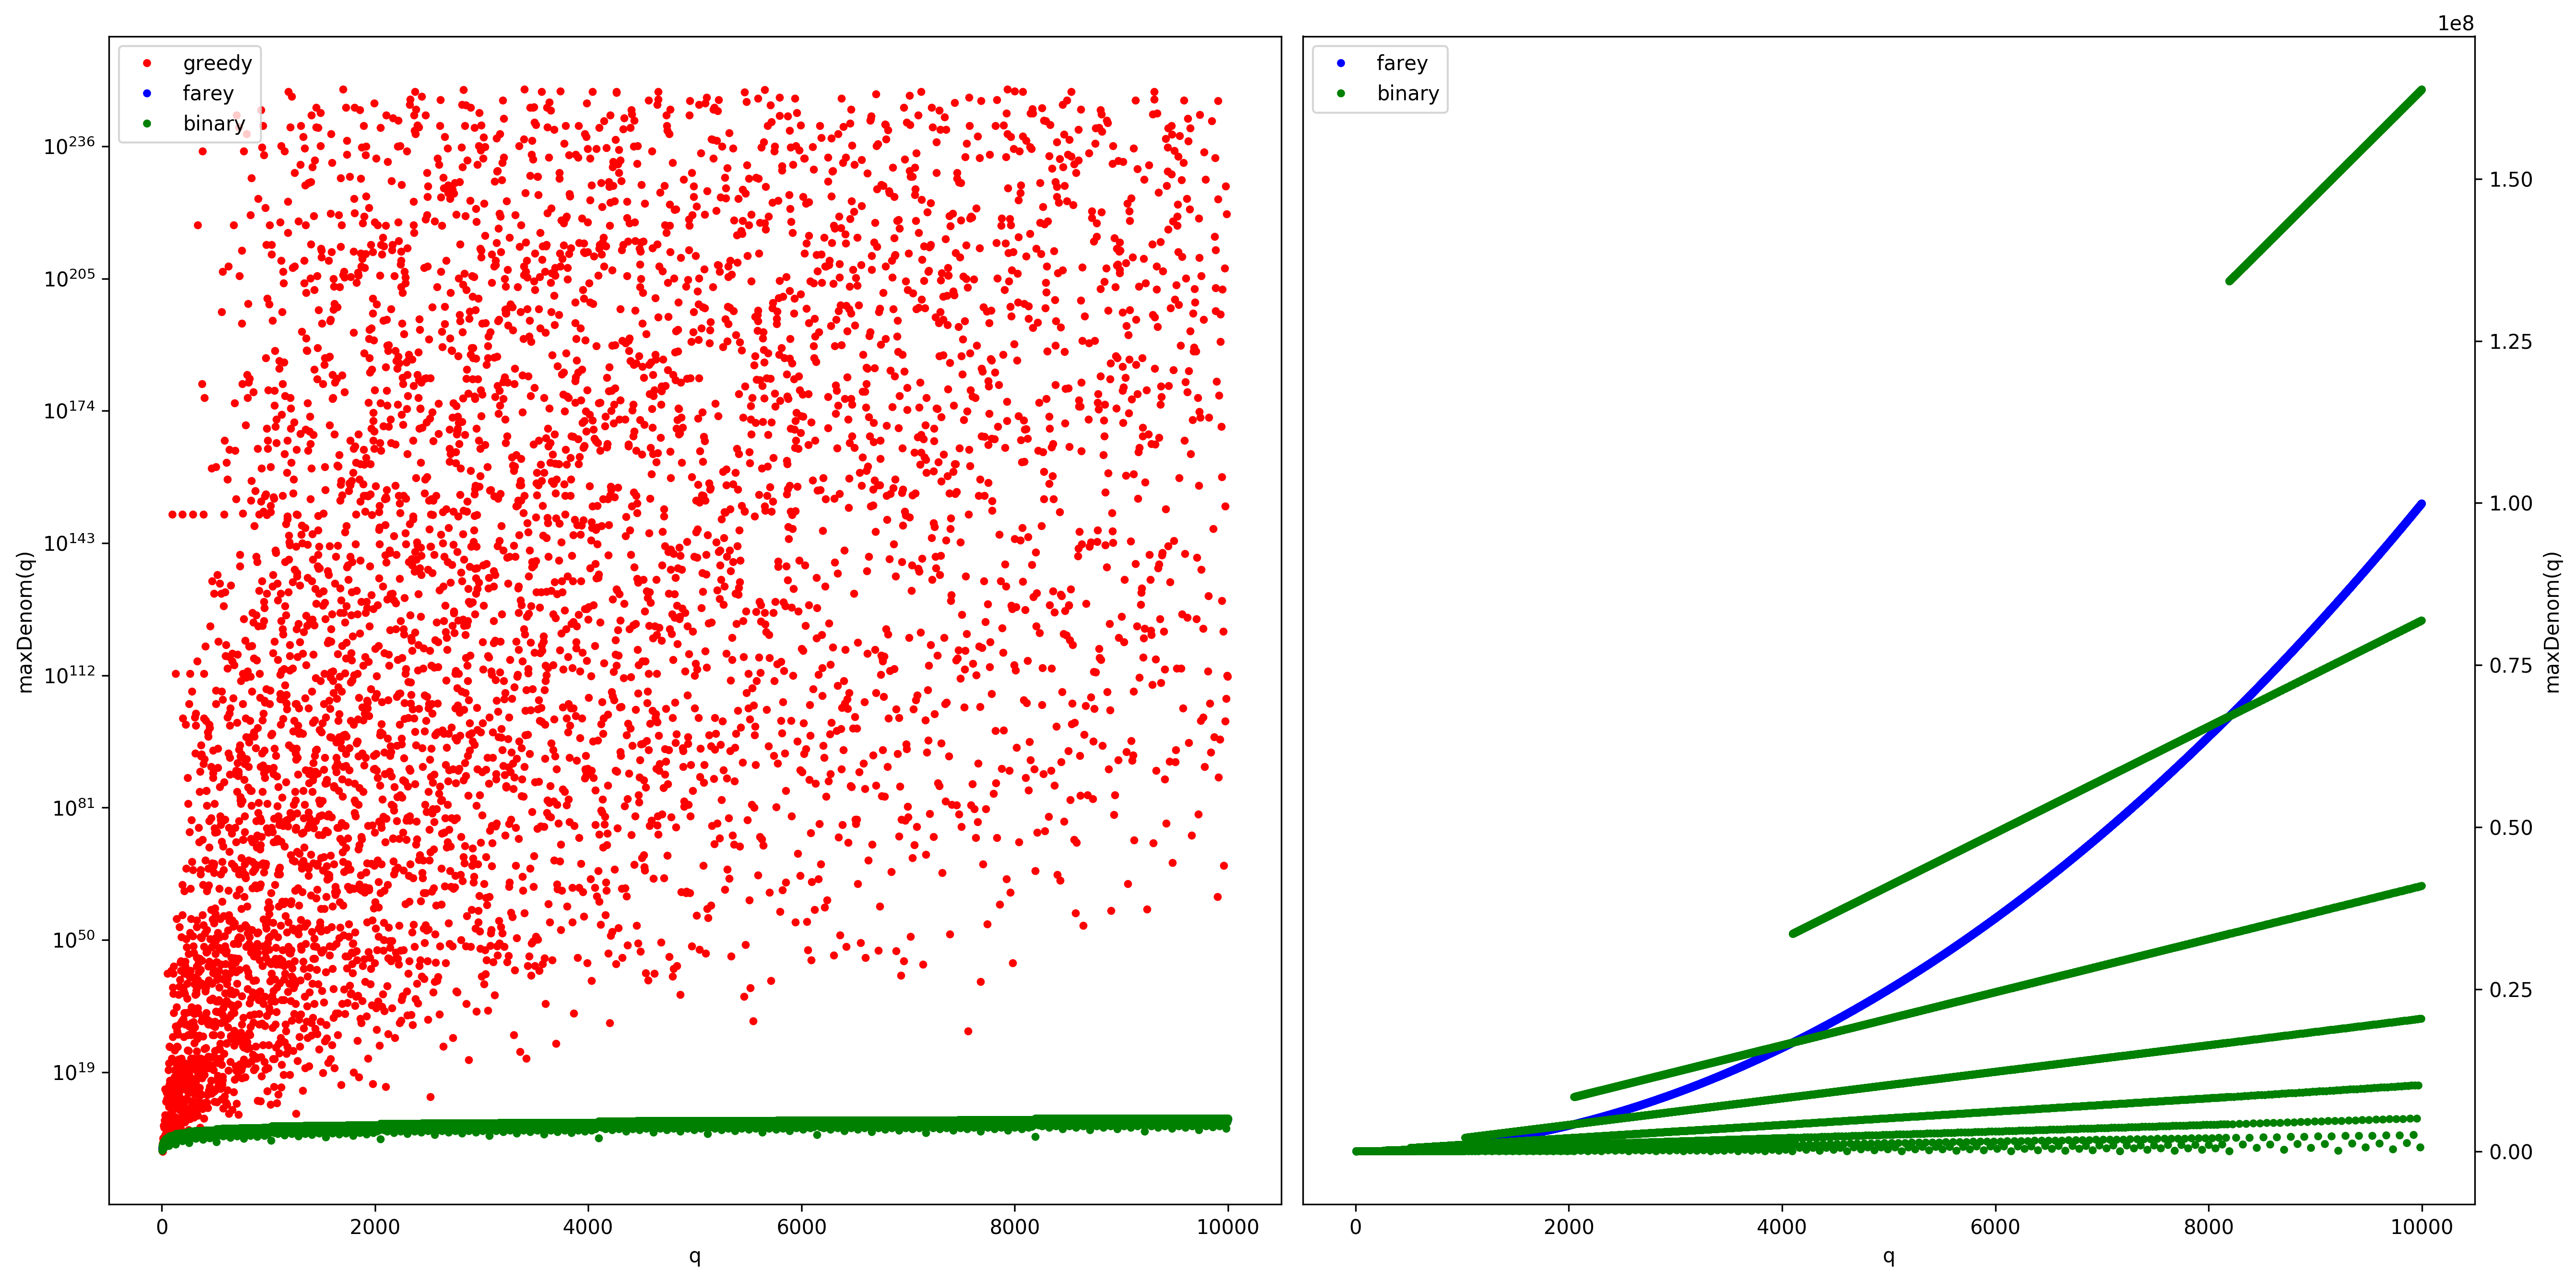
\includegraphics[width=\textwidth]{../LaTeX-Doc/images/maxDenom2in1.png}
\end{figure}
\end{frame}

\section{Theorie und Ausblick}
\subsection{Theoretische Schranken}

\begin{frame}
	\frametitle{Bekannte theoretische Schranken}
	\begin{block}{Berechnung von $\frac{2}{n}$}
	Sei $n \in \N$ ungerade. $\frac{2}{n}$ lässt sich für jedes $n$ als Summe zweier Stammbrüche notieren, nämlich:
	$$\frac{2}{n} = \uf{\lceil \frac{n}{2} \rceil} + \uf{n \cdot \lceil \frac{n}{2} \rceil}.$$
	\end{block}
	\begin{block}{Berechnung von $\frac{3}{n}$}<2->
		$$\frac{3}{n} = \uf{n} + \uf{\lceil \frac{n}{2} \rceil} + \uf{n \cdot \lceil \frac{n}{2} \rceil}.$$
	\end{block}
\end{frame}

\subsection{Ungeklärte theoretische Fragen}

\begin{frame}
	\frametitle{Sonstige Ansätze und offene Fragen}
	Weitere Ansätze und Fragen umfassen u.a.:
	\begin{itemize}
		\item Thesen für $\frac{4}{n}$, $\frac{5}{n}$ usw.
		\item allgemeingültige Schranken für
		\begin{itemize}
			\item Größe der Nenner
			\item Anzahl der Summanden
		\end{itemize}
		\item Zulassen auch negativer Terme
		\item Umgang mit Polynomen.
	\end{itemize}
\end{frame}

%%----------------------------------------------------------------------------------------
%%	PRESENTATION SLIDES
%%----------------------------------------------------------------------------------------
%
%%------------------------------------------------
%\section*{First Section} % Sections can be created in order to organize your presentation into discrete blocks, all sections and subsections are automatically printed in the table of contents as an overview of the talk
%%------------------------------------------------
%
%\subsection*{Subsection Example} % A subsection can be created just before a set of slides with a common theme to further break down your presentation into chunks
%
%\begin{frame}
%\frametitle{Paragraphs of Text}
%Sed iaculis dapibus gravida. Morbi sed tortor erat, nec interdum arcu. Sed id lorem lectus. Quisque viverra augue id sem ornare non aliquam nibh tristique. Aenean in ligula nisl. Nulla sed tellus ipsum. Donec vestibulum ligula non lorem vulputate fermentum accumsan neque mollis.\\~\\
%
%Sed diam enim, sagittis nec condimentum sit amet, ullamcorper sit amet libero. Aliquam vel dui orci, a porta odio. Nullam id suscipit ipsum. Aenean lobortis commodo sem, ut commodo leo gravida vitae. Pellentesque vehicula ante iaculis arcu pretium rutrum eget sit amet purus. Integer ornare nulla quis neque ultrices lobortis. Vestibulum ultrices tincidunt libero, quis commodo erat ullamcorper id.
%\end{frame}
%
%%------------------------------------------------
%
%\begin{frame}
%\frametitle{Bullet Points}
%\begin{itemize}
%\item Lorem ipsum dolor sit amet, consectetur adipiscing elit
%\item Aliquam blandit faucibus nisi, sit amet dapibus enim tempus eu
%\item Nulla commodo, erat quis gravida posuere, elit lacus lobortis est, quis porttitor odio mauris at libero
%\item Nam cursus est eget velit posuere pellentesque
%\item Vestibulum faucibus velit a augue condimentum quis convallis nulla gravida
%\end{itemize}
%\end{frame}
%
%%------------------------------------------------
%
%\begin{frame}
%\frametitle{Blocks of Highlighted Text}
%\begin{block}{Block 1}
%Lorem ipsum dolor sit amet, consectetur adipiscing elit. Integer lectus nisl, ultricies in feugiat rutrum, porttitor sit amet augue. Aliquam ut tortor mauris. Sed volutpat ante purus, quis accumsan dolor.
%\end{block}
%
%\begin{block}{Block 2}
%Pellentesque sed tellus purus. Class aptent taciti sociosqu ad litora torquent per conubia nostra, per inceptos himenaeos. Vestibulum quis magna at risus dictum tempor eu vitae velit.
%\end{block}
%
%\begin{block}{Block 3}
%Suspendisse tincidunt sagittis gravida. Curabitur condimentum, enim sed venenatis rutrum, ipsum neque consectetur orci, sed blandit justo nisi ac lacus.
%\end{block}
%\end{frame}
%
%%------------------------------------------------
%
%\begin{frame}
%\frametitle{Multiple Columns}
%\begin{columns}[c] % The "c" option specifies centered vertical alignment while the "t" option is used for top vertical alignment
%
%\column{.45\textwidth} % Left column and width
%\textbf{Heading}
%\begin{enumerate}
%\item Statement
%\item Explanation
%\item Example
%\end{enumerate}
%
%\column{.5\textwidth} % Right column and width
%Lorem ipsum dolor sit amet, consectetur adipiscing elit. Integer lectus nisl, ultricies in feugiat rutrum, porttitor sit amet augue. Aliquam ut tortor mauris. Sed volutpat ante purus, quis accumsan dolor.
%
%\end{columns}
%\end{frame}
%
%%------------------------------------------------
%\section*{Second Section}
%%------------------------------------------------
%
%\begin{frame}
%\frametitle{Table}
%\begin{table}
%\begin{tabular}{l l l}
%\toprule
%\textbf{Treatments} & \textbf{Response 1} & \textbf{Response 2}\\
%\midrule
%Treatment 1 & 0.0003262 & 0.562 \\
%Treatment 2 & 0.0015681 & 0.910 \\
%Treatment 3 & 0.0009271 & 0.296 \\
%\bottomrule
%\end{tabular}
%\caption{Table caption}
%\end{table}
%\end{frame}
%
%%------------------------------------------------
%
%\begin{frame}
%\frametitle{Theorem}
%\begin{theorem}[Mass--energy equivalence]
%$E = mc^2$
%\end{theorem}
%\end{frame}
%
%%------------------------------------------------
%
%\begin{frame}[fragile] % Need to use the fragile option when verbatim is used in the slide
%\frametitle{Verbatim}
%\begin{example}[Theorem Slide Code]
%\begin{verbatim}
%\begin{frame}
%\frametitle{Theorem}
%\begin{theorem}[Mass--energy equivalence]
%$E = mc^2$
%\end{theorem}
%\end{frame}\end{verbatim}
%\end{example}
%\end{frame}
%
%%------------------------------------------------
%
%\begin{frame}
%\frametitle{Figure}
%Uncomment the code on this slide to include your own image from the same directory as the template .TeX file.
%%\begin{figure}
%%\includegraphics[width=0.8\linewidth]{test}
%%\end{figure}
%\end{frame}
%
%%------------------------------------------------
%
%\begin{frame}[fragile] % Need to use the fragile option when verbatim is used in the slide
%\frametitle{Citation}
%An example of the \verb|\cite| command to cite within the presentation:\\~
%
%This statement requires citation \cite{p1}.
%\end{frame}
%
%%------------------------------------------------
%
%\begin{frame}
%\frametitle{References}
%\footnotesize{
%\begin{thebibliography}{99} % Beamer does not support BibTeX so references must be inserted manually as below
%\bibitem[Smith, 2012]{p1} John Smith (2012)
%\newblock Title of the publication
%\newblock \emph{Journal Name} 12(3), 45 -- 678.
%\end{thebibliography}
%}
%\end{frame}
%
%%------------------------------------------------
%
%\begin{frame}
%\Huge{\centerline{The End}}
%\end{frame}
%
%%----------------------------------------------------------------------------------------
%
\end{document}
